\newpage

\section{Datengrundlage und Datenvorverarbeitung}
\label{sec:datengrundlage}

\subsection{Beschreibung des Datensatzes}
\label{subsec:datensatz}

Die Datengrundlage dieser Arbeit bildet der öffentlich verfügbare Datensatz \textit{Monthly and Annual Energy Consumption by Sector} der U.S. Energy Information Administration \citeyear{datensatz}. Der Datensatz umfasst den monatlichen Energieverbrauch der letzten Jahrzehnte in den Vereinigten Staaten, aufgeschlüsselt nach Verbrauchssektoren (Residential, Commercial, Industrial, Transportation) sowie aggregiert als \textit{Total Primary Energy Consumption}. Die Einträge reichen von Januar 1973 bis Dezember 2024 und bilden eine konsistente Zeitreihe zur Analyse des Energieverbrauchsverhaltens der US-Amerikaner.

\subsection{Datenvorverarbeitung}
\label{subsec:vorverarbeitung}

Für die Analyse wurde der Datensatz als CSV-Datei lokal gespeichert und verarbeitet. Die Zielvariable ist die Spalte \texttt{Total Primary Energy Consumption}, welche den monatlichen Gesamtverbrauch aller Sektoren aggregiert und als Primärenergie abbildet. Die folgenden Vorverarbeitungsschritte erfolgten mit Hilfe der Python-Bibliothek \textit{pandas}:

\begin{itemize}
    \item Die Zeitstempel aus der Spalte \texttt{Month} wurden in ein standardisiertes \texttt{datetime}-Format (\textit{YYYY-MM}) überführt und als Tabellenindex gesetzt
    \item Die Spalte \textit{Total Primary Energy Consumption} wurde extrahiert
    \item Dezimalzahlen der Spalte, die mit einem Komma (\texttt{,}) geschrieben waren, wurden zu einem Punkt (\texttt{.}) umgewandelt
    \item Möglicherweise fehlende Werte wurden durch lineare Interpolation eingefügt
    \item Abschließend wurde die Zeitreihe auf eine monatliche Frequenz - beginnend jeden Januar - standardisiert nach aufsteigendem Datum sortiert
\end{itemize}

Die vollständige Zeitreihe wurde zur Erstellung der Prognosemodelle in Trainings- und Testdaten aufgeteilt:

\begin{itemize}
    \item \textbf{Trainingsdaten:} Daten von Januar 1973 bis einschließlich Dezember 2014 (\texttt{TRAIN\_END\_YEAR = 2014})
    \item \textbf{Testdaten:} Daten von Januar 2015 bis einschließlich Dezember 2024 (\texttt{TEST\_END\_YEAR = 2024})
\end{itemize}

Diese Aufteilung orientiert sich an der best-practice ca. 20\% der Daten zur Modellvalidierung nach dem Training zu verwenden.


\subsection{Datenexploration}
\label{subsec:exploration}

Zur Untersuchung des Primärenergieverbrauchs in den Vereinigten Staaten wurde eine umfangreiche explorative Analyse durchgeführt. Diese soll grundlegende Strukturen, Trends und Muster in der Zeitreihe identifizieren und als Grundlage für die Modellierung dienen.

\subsubsection{Zeitlicher Verlauf}
\label{subsubsec:exploration-timeseries}

Die Zeitreihe (siehe Abbildung~\ref{fig:time_series}) zeigt einen übergeordneten, langfristigen Anstieg des Energieverbrauchs über die Jahrzehnte hinweg. Deutliche saisonale Schwankungen innerhalb der Jahre lassen auf zyklische Muster schließen, die v.a. durch Temperatur und Wirtschaftsaktivität beeinflusst sein dürften.

\begin{figure}[h!]
    \centering
    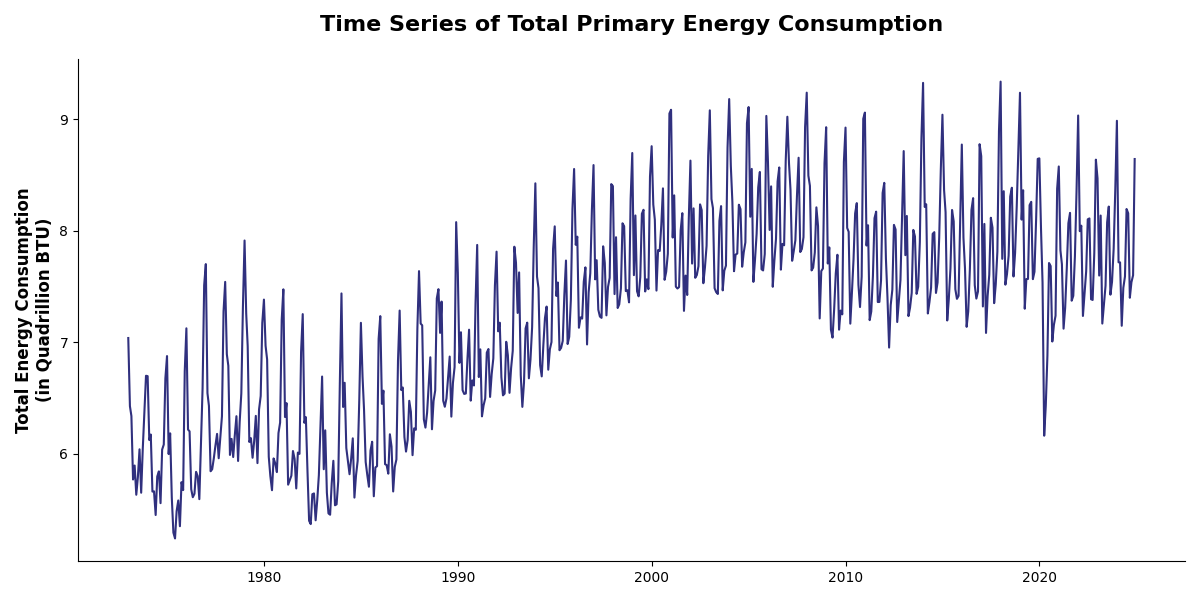
\includegraphics[width=0.9\textwidth]{images/expl/time_series.png}
    \caption{Zeitreihe des gesamten Primärenergieverbrauchs}
    \label{fig:time_series}
\end{figure}

\subsubsection{Gleitender Durchschnitt}
\label{subsubsec:exploration-moving-average}

Ein 12-monatiger gleitender Durchschnitt (Abbildung~\ref{fig:moving_average}) wurde berechnet, um kurzfristige Schwankungen zu glätten. Der geglättete Verlauf bestätigt einen strukturellen Aufwärtstrend mit Phasen moderater Stagnation, z.B. während wirtschaftlicher Krisen.

\begin{figure}[h!]
    \centering
    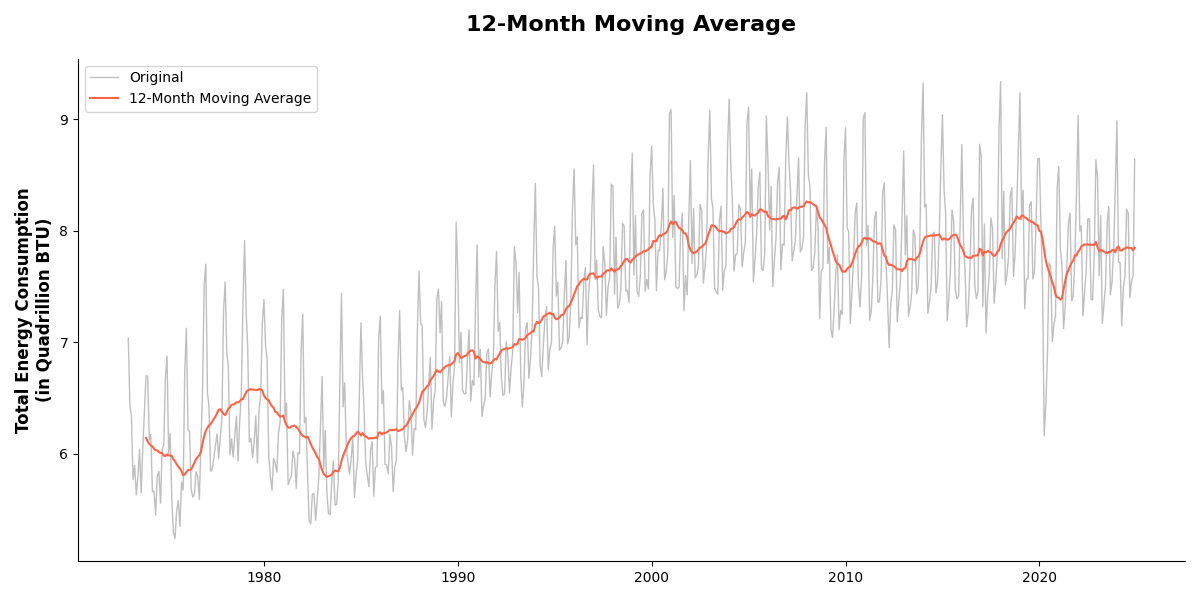
\includegraphics[width=0.9\textwidth]{images/expl/moving_average.png}
    \caption{12-Monats gleitender Durchschnitt des Energieverbrauchs}
    \label{fig:moving_average}
\end{figure}

\subsubsection{Saisonale Muster}
\label{subsubsec:exploration-seasonality}

Abbildung~\ref{fig:monthly_seasonality} zeigt den durchschnittlichen Verbrauch je Monat. Höhere Werte im Winter (Januar, Dezember) deuten auf Heizenergiebedarf hin, während die Sommermonate tendenziell niedrigere Verbräuche aufweisen.

\begin{figure}[h!]
    \centering
    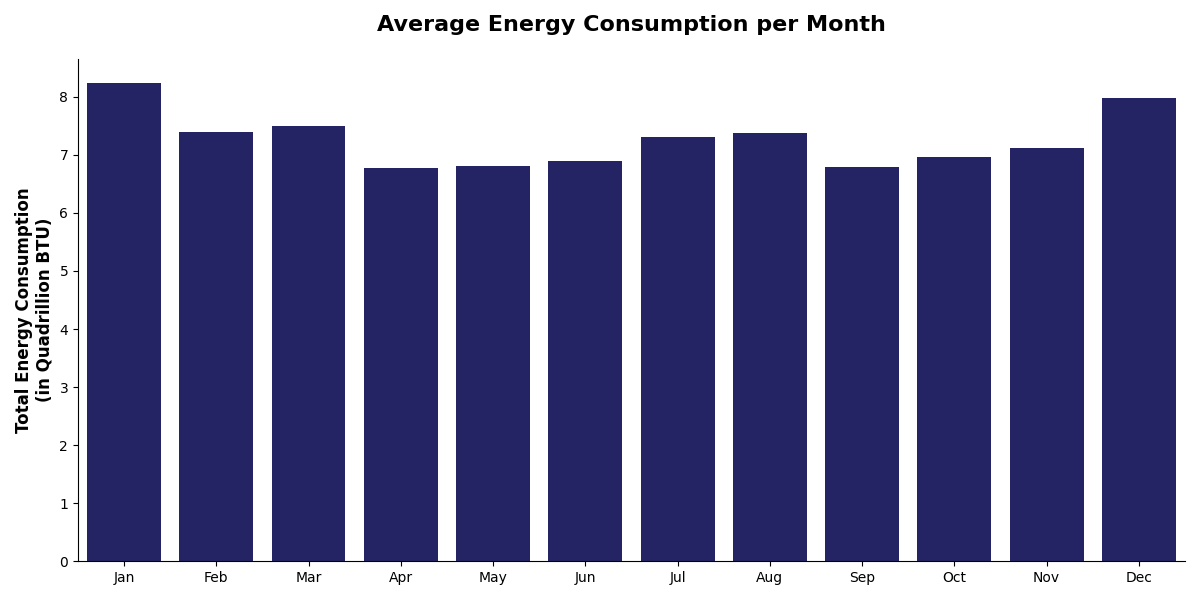
\includegraphics[width=0.9\textwidth]{images/expl/monthly_seasonality.png}
    \caption{Durchschnittlicher Energieverbrauch pro Monat}
    \label{fig:monthly_seasonality}
\end{figure}

Auch der Boxplot nach Monaten (Abbildung~\ref{fig:boxplot_by_month}) verdeutlicht die Streuung innerhalb der Monate und zeigt, dass insbesondere im Winter höhere und variablere Werte auftreten.

\begin{figure}[h!]
    \centering
    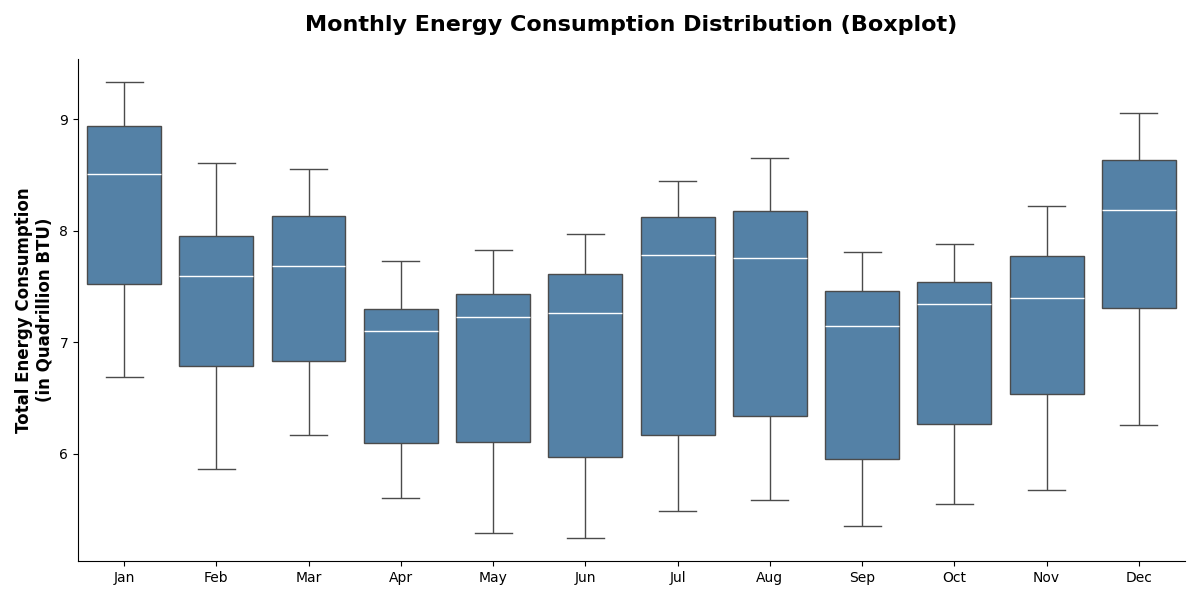
\includegraphics[width=0.9\textwidth]{images/expl/boxplot_by_month.png}
    \caption{Monatliche Verteilung des Energieverbrauchs (Boxplot)}
    \label{fig:boxplot_by_month}
\end{figure}

\subsubsection{Zerlegung der Zeitreihe}
\label{subsubsec:exploration-decomposition}

Eine additive Zerlegung (Abbildung~\ref{fig:decomposition}) teilt die Zeitreihe in Trend-, Saison- und Residualkomponenten. Die Saisonalität zeigt ein stark regelmäßiges Muster, während der Trend die langfristige Entwicklung nachzeichnet. Die Residuen erscheinen relativ zufällig verteilt.

\begin{figure}[h!]
    \centering
    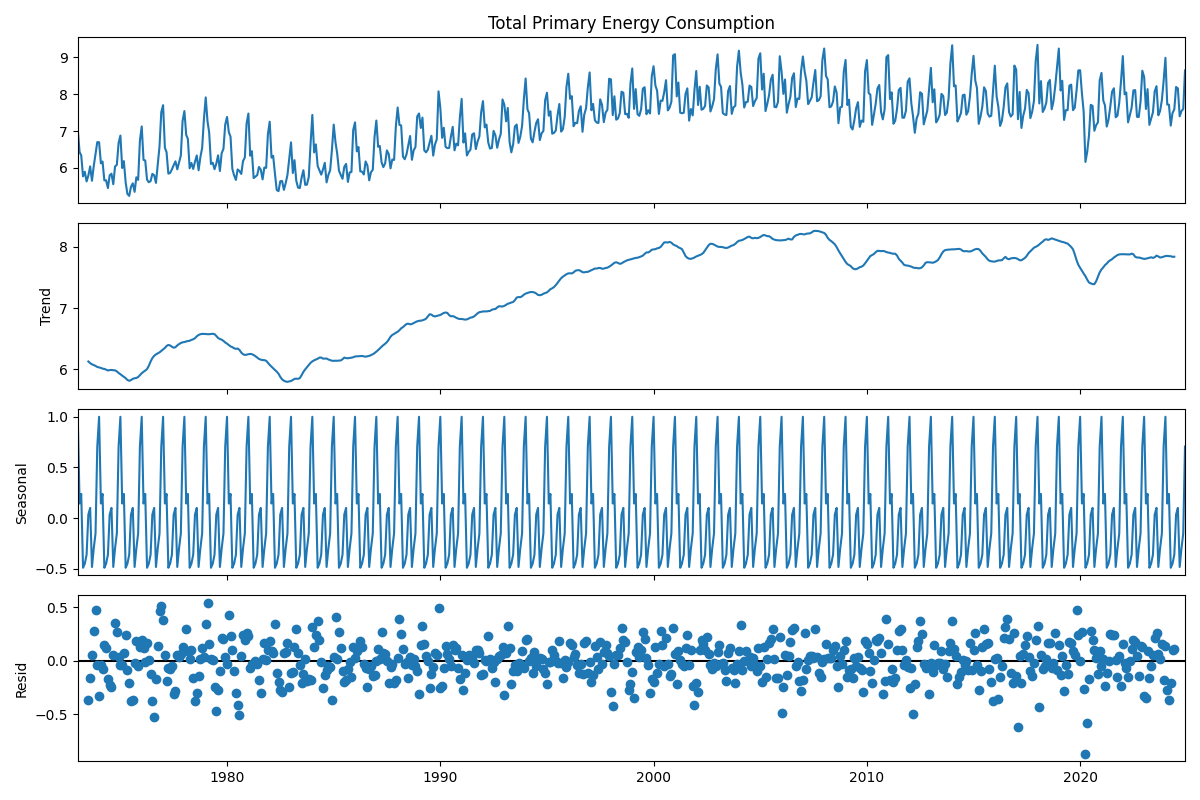
\includegraphics[width=0.95\textwidth]{images/expl/decomposition_additive.png}
    \caption{Additive Zeitreihen-Zerlegung}
    \label{fig:decomposition}
\end{figure}

\subsubsection{Verteilungsanalyse}
\label{subsubsec:exploration-distribution}

Das Histogramm (Abbildung~\ref{fig:histogram}) zeigt eine leicht rechtsschiefe Verteilung mit einer Häufung im Bereich 7–8 Quadrillion BTU. Extremwerte oberhalb von 9 deuten auf besonders verbrauchsintensive Phasen hin.

\begin{figure}[h!]
    \centering
    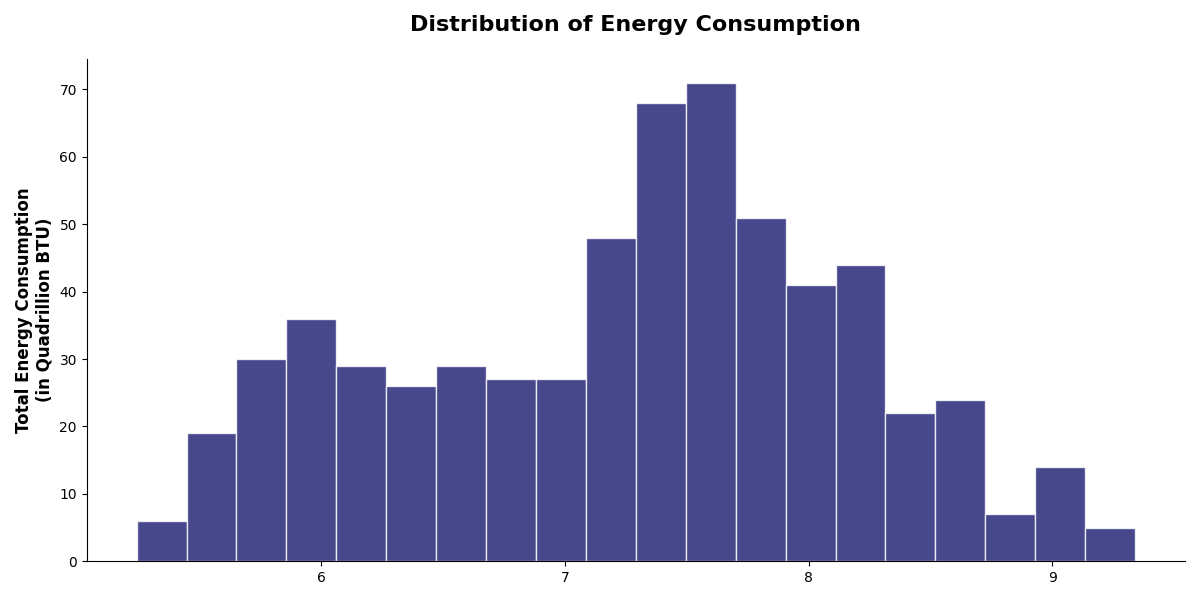
\includegraphics[width=0.9\textwidth]{images/expl/histogram.png}
    \caption{Verteilung des Energieverbrauchs}
    \label{fig:histogram}
\end{figure}

\subsubsection{Autokorrelation}
\label{subsubsec:exploration-acf}

Die Autokorrelationsanalyse (Abbildung~\ref{fig:acf_pacf}) zeigt signifikante Korrelationen über mehr als 36 Monate hinweg. Die PACF deutet auf eine autoregressive Struktur mit mehreren signifikanten Lags hin – u.a. bei Lag 1, 3, 6 und 12, was typische saisonale Muster bestätigt.

\begin{figure}[h!]
    \centering
    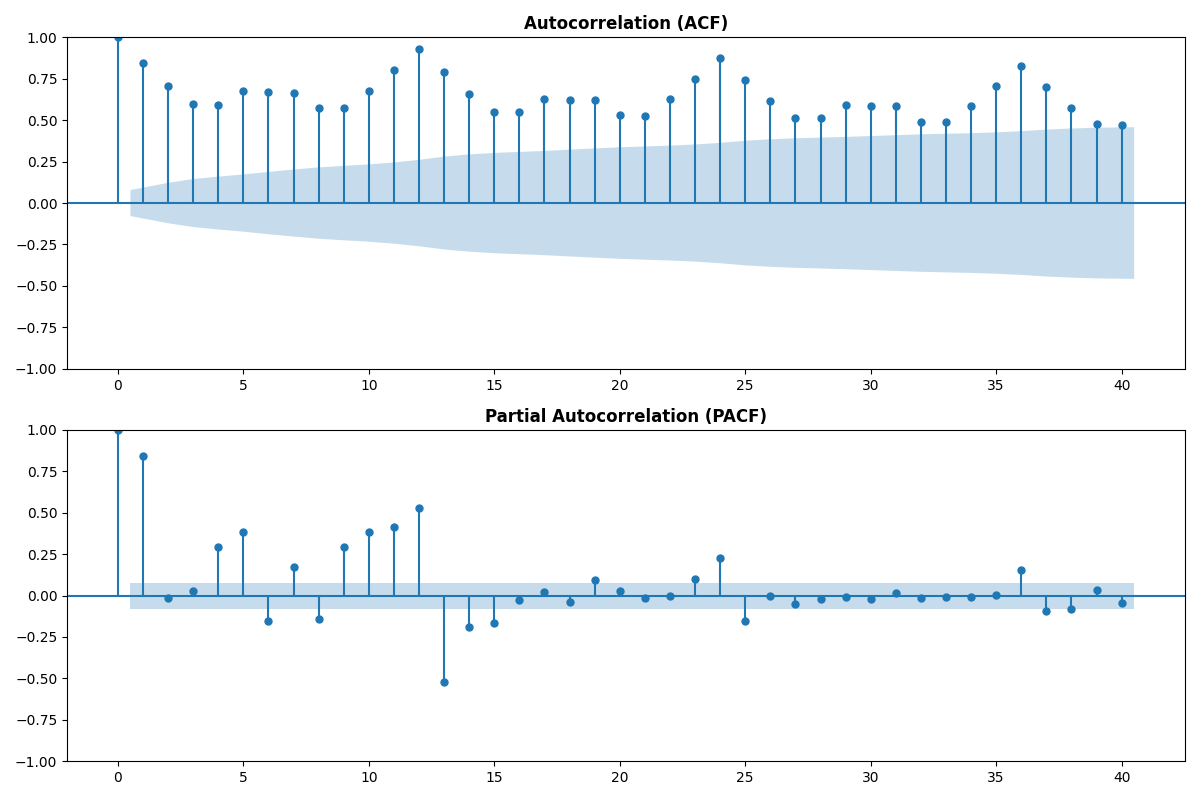
\includegraphics[width=0.95\textwidth]{images/expl/acf_pacf.png}
    \caption{Autokorrelation (ACF) und partielle Autokorrelation (PACF)}
    \label{fig:acf_pacf}
\end{figure}
